\documentclass[12pt,utf8,notheorems,compress,t]{beamer}
\usepackage{etex}

\usepackage[english]{babel}

\usepackage{mathtools}
\usepackage{booktabs}
\usepackage{stmaryrd}
\usepackage{array}
\usepackage{ragged2e}
\usepackage{multicol}
\usepackage{tabto}
\usepackage{xstring}
\usepackage{ifthen}
\usepackage{soul}\setul{0.3ex}{}
\usepackage[all]{xy}
\xyoption{rotate}
\usepackage{tikz}
\usetikzlibrary{calc,shapes,shapes.callouts,shapes.arrows,patterns,fit,backgrounds,decorations.pathmorphing}
\hypersetup{colorlinks=true}
\usepackage{multimedia}
\newcommand{\video}[2]{\movie[width=#2,height=#2,autostart,loop,poster]{}{#1}}
\hypersetup{colorlinks=false}

\usepackage{pifont}
\newcommand{\cmark}{\ding{51}}
\newcommand{\xmark}{\ding{55}}
\DeclareSymbolFont{extraup}{U}{zavm}{m}{n}
\DeclareMathSymbol{\varheart}{\mathalpha}{extraup}{86}

\graphicspath{{images/}}

\usepackage[protrusion=true,expansion=true]{microtype}

\setlength\parskip{\medskipamount}
\setlength\parindent{0pt}

\title{New reduction techniques in commutative algebra driven by logical methods}
\author{Ingo Blechschmidt}
\date{September 15th, 2018}

\useinnertheme[shadow=true]{rounded}
\useoutertheme[subsection=false]{miniframes}
\setbeamerfont{block title}{size={}}

\useinnertheme{rectangles}

\usecolortheme{orchid}
\usecolortheme{seahorse}
\definecolor{mypurple}{RGB}{150,0,255}
\setbeamercolor{structure}{fg=mypurple}
\definecolor{myred}{RGB}{150,0,0}
\setbeamercolor*{title}{bg=myred,fg=white}
\setbeamercolor*{titlelike}{bg=myred,fg=white}
\setbeamercolor{frame}{bg=black}

\usefonttheme{serif}
\usepackage[T1]{fontenc}
\usepackage{libertine}

\newcommand{\A}{\mathcal{A}}
\renewcommand{\AA}{\mathbb{A}}
\newcommand{\E}{\mathcal{E}}
\newcommand{\F}{\mathcal{F}}
\renewcommand{\G}{\mathcal{G}}
\newcommand{\GG}{\mathbb{G}}
\renewcommand{\O}{\mathcal{O}}
\newcommand{\K}{\mathcal{K}}
\newcommand{\NN}{\mathbb{N}}
\newcommand{\QQ}{\mathbb{Q}}
\newcommand{\RR}{\mathbb{R}}
\newcommand{\TT}{\mathbb{T}}
\newcommand{\PP}{\mathbb{P}}
\newcommand{\ZZ}{\mathbb{Z}}
\renewcommand{\P}{\mathcal{P}}
\newcommand{\ppp}{\mathfrak{p}}
\newcommand{\defeq}{\vcentcolon=}
\newcommand{\defeqv}{\vcentcolon\equiv}
\newcommand{\Sh}{\mathrm{Sh}}
\newcommand{\GL}{\mathrm{GL}}
\newcommand{\Zar}{\mathrm{Zar}}
\newcommand{\op}{\mathrm{op}}
\newcommand{\Set}{\mathrm{Set}}
\newcommand{\Eff}{\mathrm{Ef{}f}}
\newcommand{\Sch}{\mathrm{Sch}}
\newcommand{\Aff}{\mathrm{Aff}}
\newcommand{\LRS}{\mathrm{LRS}}
\newcommand{\Hom}{\mathrm{Hom}}
\newcommand{\Spec}{\mathrm{Spec}}
\newcommand{\lra}{\longrightarrow}
\newcommand{\RelSpec}{\operatorname{Spec}}
\renewcommand{\_}{\mathpunct{.}}
\newcommand{\?}{\,{:}\,}
\newcommand{\speak}[1]{\ulcorner\text{\textnormal{#1}}\urcorner}
\newcommand{\ull}[1]{\underline{#1}}
\newcommand{\affl}{\ensuremath{{\ull{\AA}^1}}}
\newcommand{\Ll}{\vcentcolon\!\Longleftrightarrow}
\newcommand{\inv}{inv.\@}
\newcommand{\seq}{\vdash_{\!\!\!\vec x}}

\setbeamertemplate{blocks}[rounded][shadow=false]

% Adapted from https://latex.org/forum/viewtopic.php?t=2251 (Stefan Kottwitz)
\newenvironment<>{hilblock}{
  \begin{center}
    \begin{minipage}{9.05cm}
      \setlength{\textwidth}{9.05cm}
      \begin{actionenv}#1
        \def\insertblocktitle{}
        \par
        \usebeamertemplate{block begin}}{
        \par
        \usebeamertemplate{block end}
      \end{actionenv}
    \end{minipage}
  \end{center}}

\newcommand{\bignumber}[1]{
  \renewcommand{\insertenumlabel}{#1}\scalebox{1.5}{\usebeamertemplate{enumerate item}}
}
\newcommand{\bigheart}[1]{\scalebox{1.5}{\hil{$\varheart$}}}

\newenvironment{changemargin}[2]{%
  \begin{list}{}{%
    \setlength{\topsep}{0pt}%
    \setlength{\leftmargin}{#1}%
    \setlength{\rightmargin}{#2}%
    \setlength{\listparindent}{\parindent}%
    \setlength{\itemindent}{\parindent}%
    \setlength{\parsep}{\parskip}%
  }%
  \item[]}{\end{list}}

\tikzset{
  invisible/.style={opacity=0,text opacity=0},
  visible on/.style={alt={#1{}{invisible}}},
  alt/.code args={<#1>#2#3}{%
    \alt<#1>{\pgfkeysalso{#2}}{\pgfkeysalso{#3}}}
}

\newcommand{\pointthis}[3]{%
  \tikz[remember picture,baseline]{
    \node[anchor=base,inner sep=0,outer sep=0] (#2) {#2};
    \node[visible on=#1,overlay,rectangle callout,rounded corners,callout relative pointer={(0.3cm,0.5cm)},fill=blue!20] at ($(#2.north)+(-0.1cm,-1.1cm)$) {#3};
  }%
}

% Adapted from https://latex.org/forum/viewtopic.php?t=2251 (Stefan Kottwitz)
\newenvironment<>{varblock}[2]{
  \begin{center}
    \begin{minipage}{#1}
      %\setlength{\textwidth}{#1}
      \begin{actionenv}#3
	\def\insertblocktitle{\centering #2}
	\par
	\usebeamertemplate{block begin}}{
        \par
        \usebeamertemplate{block end}
      \end{actionenv}
    \end{minipage}
  \end{center}}

\setbeamertemplate{frametitle}{%
  \vskip0.7em%
  \leavevmode%
  \begin{beamercolorbox}[dp=1ex,center]{}%
      \usebeamercolor[fg]{item}{\textbf{{\Large \insertframetitle}}}
  \end{beamercolorbox}%
}

\setbeamertemplate{navigation symbols}{}

\newcounter{framenumberpreappendix}
\newcommand{\backupstart}{
  \setcounter{framenumberpreappendix}{\value{framenumber}}
}
\newcommand{\backupend}{
  \addtocounter{framenumberpreappendix}{-\value{framenumber}}
  \addtocounter{framenumber}{\value{framenumberpreappendix}} 
}

\setbeamertemplate{headline}{%
  \begin{beamercolorbox}[wd=\paperwidth,ht=2.25ex]{}%
    \insertnavigation{\paperwidth}%
  \end{beamercolorbox}%
  \vskip0pt%
}

\setbeamertemplate{footline}{%
  \begin{beamercolorbox}[wd=\paperwidth,ht=2.25ex,dp=1ex,right,rightskip=1mm,leftskip=1mm]{}%
    % \inserttitle
    \hfill
    \insertframenumber\,/\,\inserttotalframenumber
  \end{beamercolorbox}%
  \vskip0pt%
}


\newcommand{\hil}[1]{{\usebeamercolor[fg]{item}{\textbf{#1}}}}
\newcommand{\bad}[1]{\textcolor{red!90}{\textnormal{#1}}}

\begin{document}

\addtocounter{framenumber}{-1}

{\usebackgroundtemplate{\begin{minipage}{\paperwidth}\vspace*{4.95cm}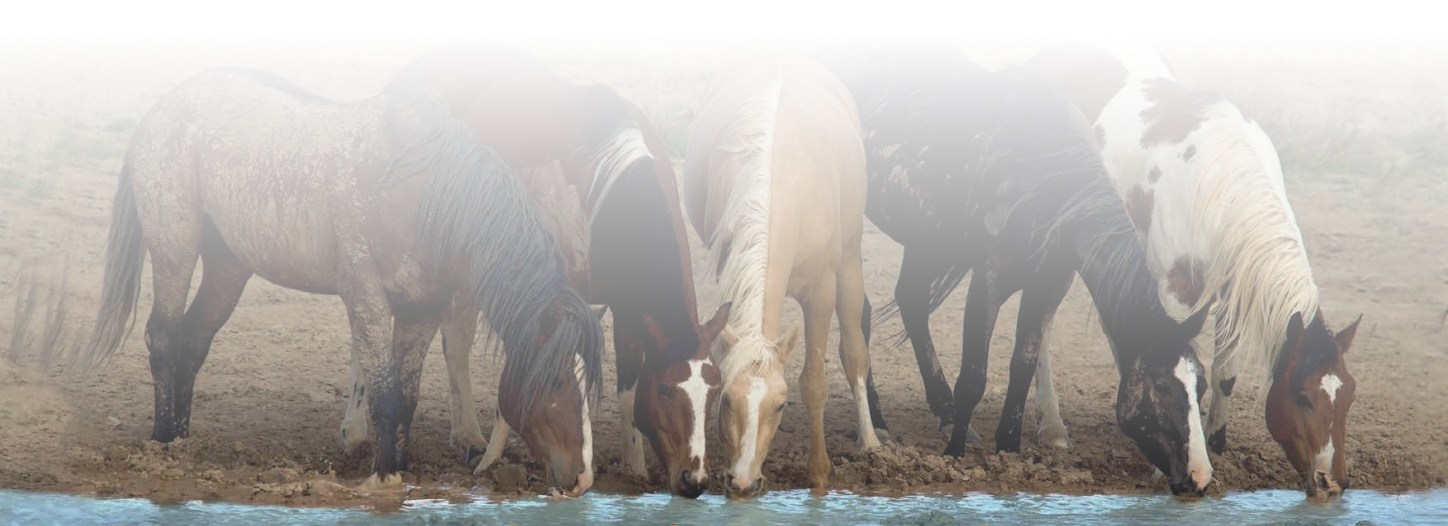
\includegraphics[width=\paperwidth]{topos-horses}\end{minipage}}
\begin{frame}[c]
  \centering

  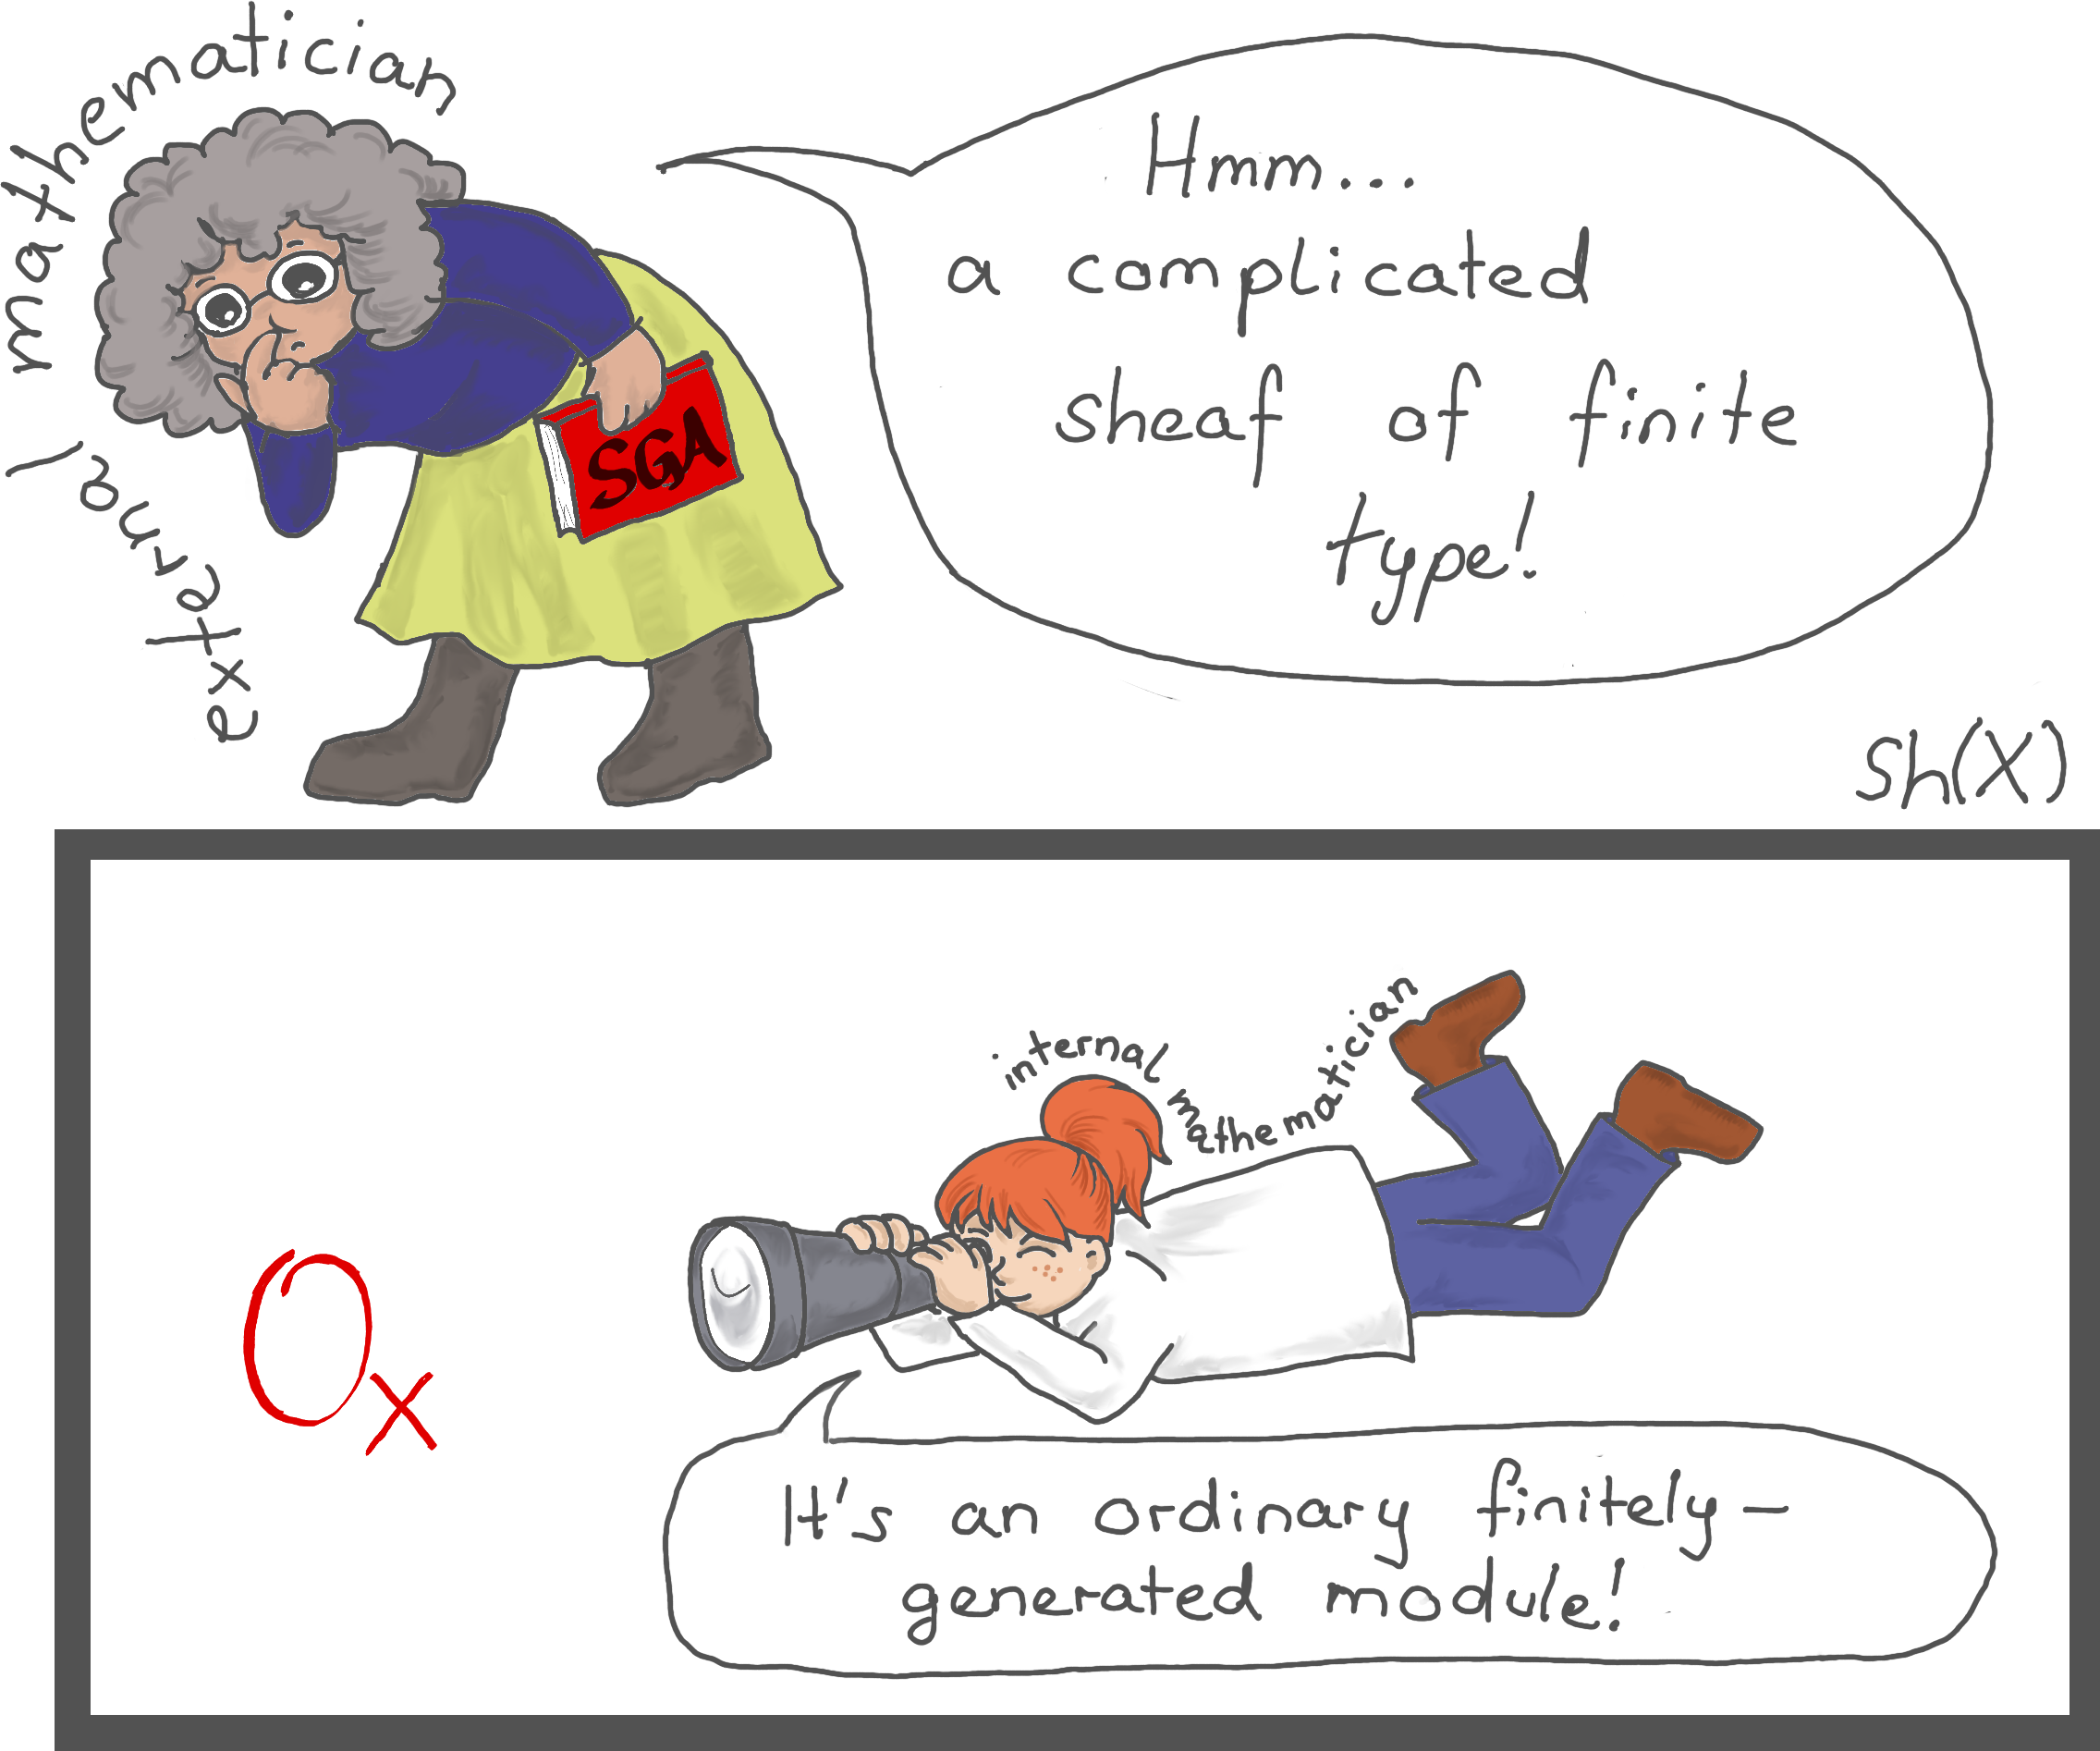
\includegraphics[width=0.4\textwidth]{external-internal}
  \bigskip

  \hil{New reduction techniques in commutative algebra driven by logical methods}

  \bigskip

  \scriptsize
  Ingo Blechschmidt \\
  University of Verona
  \bigskip

  Colloquium Logicum 2018 in Bayreuth \\
  September 15th, 2018
  \par
\end{frame}}


\section{Summary}

\begin{frame}{Summary}
  \vspace*{-1em}

  \begin{changemargin}{-2.0em}{-0.5em}
    \begin{itemize}
      \item \ \\[-1.2em]\mbox{For any reduced ring~$A$, there is a ring~$A^\sim$ in a certain topos with}
      \[ \models \bigl(\forall x\?A^\sim\_ \neg(\exists y\?A^\sim\_ xy = 1) \Rightarrow x = 0\bigr). \]

      \item This semantics is sound with respect to intuitionistic logic.

      \item \ \\[-1.2em]\mbox{It has uses in classical and constructive commutative
      algebra.}
    \end{itemize}
  \end{changemargin}

  \vspace*{-2em}

  \begin{columns}[t]
    \begin{column}[t]{0.55\textwidth}
      \centering

      \begin{varblock}{\textwidth}{A baby application}
        \justifying
        Let~$M$ be an injective matrix with more columns than rows over a ring~$A$.
        Then~$1 = 0$ in~$A$.
      \end{varblock}

      \only<1>{
        \scalebox{0.8}{$\begin{pmatrix}
          \cdot & \cdot & \cdot & \cdot & \cdot \\
          \cdot & \cdot & \cdot & \cdot & \cdot \\
          \cdot & \cdot & \cdot & \cdot & \cdot
        \end{pmatrix}$}
      }

      \visible<2>{
        \justifying
        \textbf{Proof.} \bad{Assume not.} Then there is a \bad{minimal
        prime ideal} $\ppp$. The matrix is injective over the field~$A_\ppp = A[(A
        \setminus \ppp)^{-1}]$. This is a contradiction to basic linear algebra.
      }
    \end{column}

    \begin{column}[t]{0.46\textwidth}
      \centering

      \begin{varblock}{\textwidth}{Generic freeness\phantom{p}}
        \justifying
        Generically, any finitely generated module over a reduced ring is free.
      \end{varblock}
      \vspace*{-0.5em}

      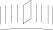
\includegraphics[width=0.6\textwidth]{generic-freeness}

      \visible<2>{
        \justifying
        \textbf{Proof.} See [Stacks Project].
      }
    \end{column}
  \end{columns}
\end{frame}


\section{The forcing model}

\begin{frame}{The little Zariski topos of a ring}
  Let~$A$ be a reduced commutative ring ($x^n = 0 \Rightarrow x = 0$).

  The \hil{little Zariski topos} of~$A$ is equivalently
  \vspace*{-0.5em}
  \begin{itemize}
    \item the topos of sheaves over~$\Spec(A)$,
    \item the classifying topos of local localizations of~$A$ or
    \item the classifying topos of prime filters of~$A$
  \end{itemize}
  \vspace*{-0.5em}
  and contains a \hil{mirror image} of~$A$, the sheaf of rings $A^\sim$.

  \vspace*{-1.5em}
  \small

  \begin{columns}
    \begin{column}{0.5\textwidth}
      \begin{varblock}{\textwidth}{}
        \justifying
        Assuming the Boolean prime ideal theorem, a first-order
        formula ``$\forall \ldots \forall\_ (\cdots \Longrightarrow \cdots\!\,)$'',
        where the two subformulas may not contain~``$\Rightarrow$'' and~``$\forall$'',
        holds for~$A^\sim$ iff it holds for all stalks~$A_\ppp$.
      \end{varblock}
    \end{column}

    \begin{column}{0.5\textwidth}
      \begin{varblock}{\textwidth}{}
        $A^\sim$ inherits any property of~$A$ which is
        \hil{localization-stable}.
      \end{varblock}

      \vspace*{-1.7em}

      \setbeamercolor{block body}{bg=red!30}
      \setbeamercolor{structure}{fg=purple}
      \begin{varblock}{\textwidth}{}
        $A^\sim$ is a \hil{local ring} and a \hil{field}.

        $A^\sim$ has \hil{$\boldsymbol{\neg\neg}$-stable equality}.

        \mbox{$A^\sim$ is \hil{anonymously Noetherian}.}\\[-1.2em]
      \end{varblock}
    \end{column}
  \end{columns}

  \visible<2>{\begin{tikzpicture}[overlay]
    \draw[fill=white, draw=white, opacity=0.95] (-1,0) rectangle (\paperwidth,7.4);
    \node[anchor=south west,inner sep=0] (image) at (0,0.8) {\vbox{
      \centering
      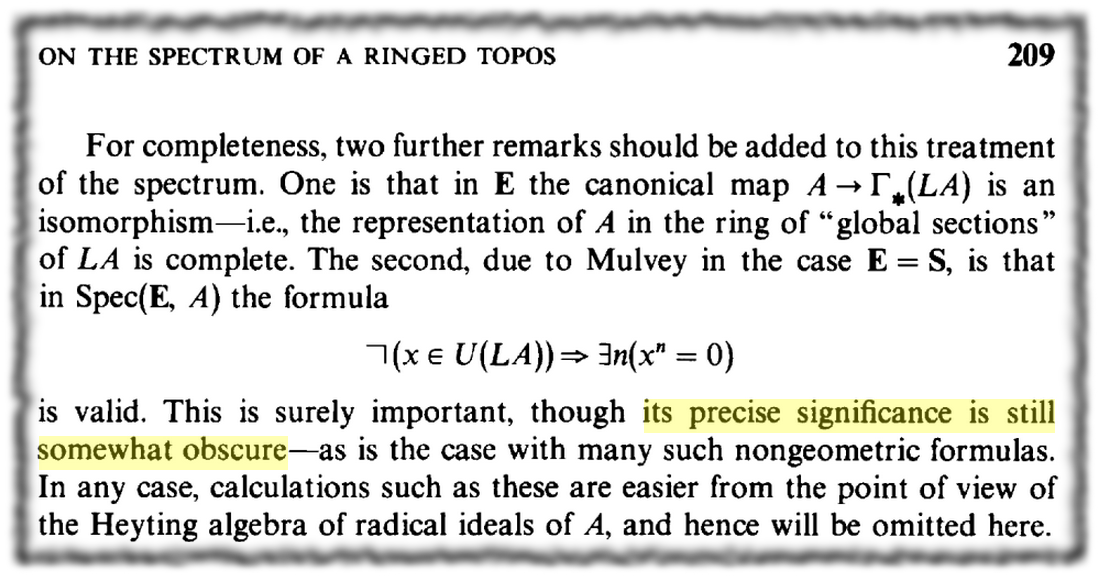
\includegraphics[width=0.9\textwidth]{tierney-on-the-spectrum-of-a-ringed-topos} \\
      \footnotesize
      Miles Tierney. On the spectrum of a ringed topos. 1976.
    }};
  \end{tikzpicture}}
\end{frame}

\begin{frame}{The Kripke--Joyal semantics for the little Zariski topos}
  \small
  \mbox{\!\!\!Recall~$A[f^{-1}] = \bigl\{ \frac{u}{f^n} \,|\, u \in A, n \in \NN \bigr\}$.
  Let~``$\models \varphi$'' be a short for~``$1 \models \varphi$''.}
  \[ \renewcommand{\arraystretch}{1.25}\begin{array}{@{}l@{\quad}c@{\quad}l@{}}
    f \models \top &\text{iff}& \top \\
    f \models \bot &\text{iff}& \text{$f$ is nilpotent} \\
    f \models x = y &\text{iff}& x = y \in A[f^{-1}] \\
    f \models \varphi \wedge \psi &\text{iff}&
      \text{$f \models \varphi$ and $f \models \psi$} \\
    f \models \varphi \vee \psi &\text{iff}&
      \text{there exists a partition~$f^n = fg_1 + \cdots + fg_m$ with,} \\
    &&\quad\text{for each~$i$, $fg_i \models \varphi$ or $fg_i \models \psi$} \\
    f \models \varphi \Rightarrow \psi &\text{iff}&
      \text{for all~$g \in A$, $fg \models \varphi$ implies $fg \models \psi$} \\
    f \models \forall x\?A^\sim\_ \varphi &\text{iff}&
      \text{for all~$g \in A$ and $x_0 \in A[(fg)^{-1}]$, $fg \models \varphi[x_0/x]$} \\
    f \models \exists x\?A^\sim\_ \varphi &\text{iff}&
      \text{there exists a partition~$f^n = fg_1 + \cdots + fg_m$ with,} \\
    &&\quad\text{for each~$i$, $fg_i \models \varphi[x_0/x]$ for some~$x_0 \in A[(fg_i)^{-1}]$}
  \end{array} \]
\end{frame}


\section{Revisiting the test cases}

\begin{frame}{Revisiting the test cases}
  \vspace*{-1em}
  Let~$A$ be a reduced commutative ring ($x^n = 0 \Rightarrow x = 0$). \\
  Let~$A^\sim$ be its mirror image in the little Zariski topos.

  \begin{columns}[t]
    \begin{column}[t]{0.46\textwidth}
      \centering

      \scalebox{0.5}{$\begin{pmatrix}
        \cdot & \cdot & \cdot & \cdot & \cdot \\
        \cdot & \cdot & \cdot & \cdot & \cdot \\
        \cdot & \cdot & \cdot & \cdot & \cdot
      \end{pmatrix}$}
      \vspace*{-1em}

      \begin{varblock}{\textwidth}{A baby application}
        \justifying
        Let~$M$ be an injective matrix over~$A$ with more columns than rows.
        Then~$1 = 0$ in~$A$.
      \end{varblock}

      \justifying
      \textbf{Proof.} $M$ is also injective as a matrix over~$A^\sim$.
      Since~$A^\sim$ is a field, we have~$1 = 0$ in~$A^\sim$ by basic linear
      algebra. This amounts to~$1 = 0$ in~$A$.
    \end{column}

    \begin{column}[t]{0.58\textwidth}
      \centering

      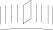
\includegraphics[height=1.9em]{generic-freeness}
      \vspace*{-1em}

      \begin{varblock}{\textwidth}{Generic freeness\phantom{p}}
        \justifying
        Let~$M$ be a finitely generated~$A$-module.
        If~$f = 0$ is the only element of~$A$ such that~$M[f^{-1}]$ is a
        free~$A[f^{-1}]$-module, then~$1 = 0$ in~$A$.
      \end{varblock}
      \vspace*{-0.1em}

      \justifying
      \textbf{Proof.} The claim amounts to \mbox{$\models
      \text{``$M^\sim$}$}$\text{
      is \hil{not not} free''}$. Since~$A^\sim$ is a field, this follows from
      basic linear algebra.
    \end{column}
  \end{columns}
\end{frame}


\backupstart

\section*{Appendix}

\begin{frame}{Vision for the future}
  \begin{columns}
    \small
    \begin{column}{0.35\textwidth}
      \centering
      \bigheart
      \par

      constructive algebra \\
      conceptual proofs \\
      proof assistants
    \end{column}

    \begin{column}{0.47\textwidth}
      \centering
      \bigheart
      \par

      constructive algebraic geometry \\
      synthetic algebraic geometry \\
      intersection theory \\
      derived categories
    \end{column}

    \begin{column}{0.25\textwidth}
      \centering
      \bigheart
      \par

      quasicoherence \\
      nongeometric mysteries \\
      further fields
    \end{column}
  \end{columns}

  \vfill

  \centering
  \href{https://www.oliviacaramello.com/Papers/Papers.htm}{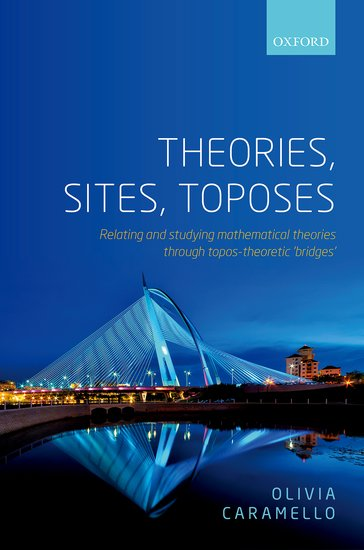
\includegraphics[height=0.45\textheight]{olivia-tst}}
  \href{http://math.andrej.com/2014/03/04/intuitionistic-mathematics-and-realizability-in-the-physical-world/}{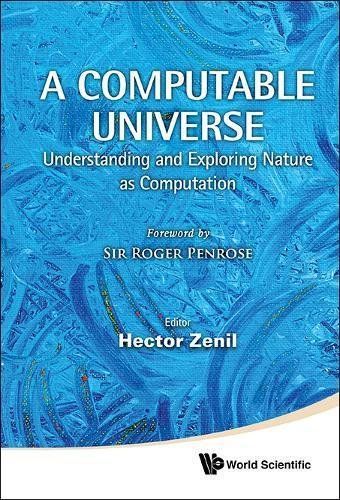
\includegraphics[height=0.45\textheight]{zenil-computable-universe}}
  \href{https://pizzaseminar.speicherleck.de/skript2/zariski-topos-klein.pdf}{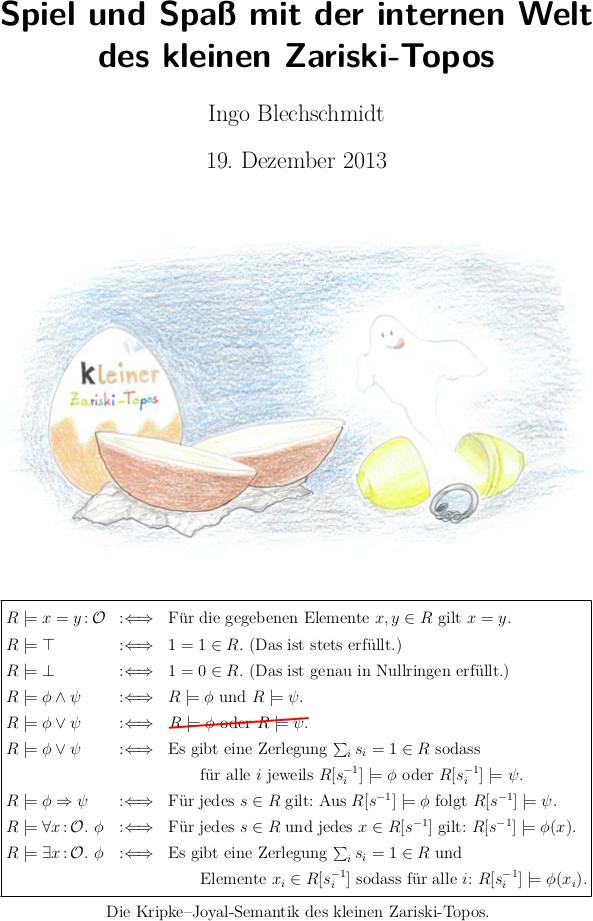
\includegraphics[height=0.45\textheight]{fun-with-the-zariski-topos}}
  \href{https://rawgit.com/iblech/internal-methods/master/notes.pdf}{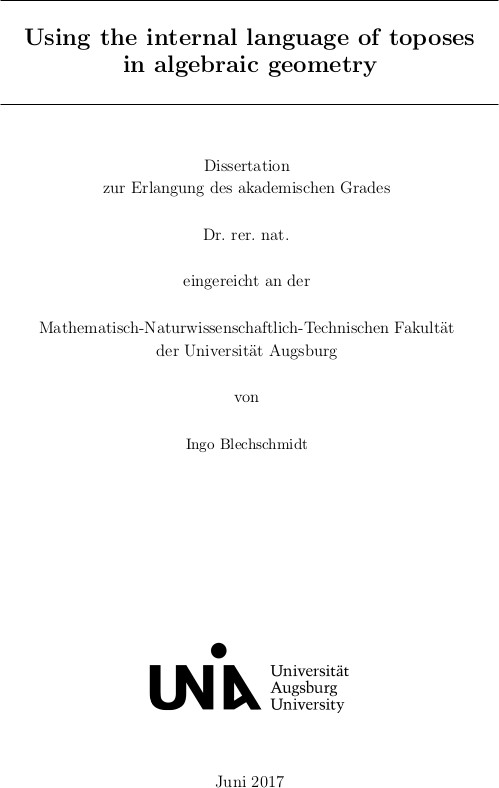
\includegraphics[height=0.45\textheight]{phd-cover}}
\end{frame}

\begin{frame}{Applications in algebraic geometry}
  \vspace*{-1.5em}
  \begin{varblock}{0.9\textwidth}{}
    \justifying
    Understand notions of algebraic geometry over a scheme~$X$ as
    notions of algebra internal to~$\Sh(X)$.
  \end{varblock}

  \small\centering
  \scalebox{0.83}{\begin{tabular}{ll}
    \toprule
    externally & internally to $\Sh(X)$ \\
    \midrule
    sheaf of sets & set \\
    %sheaf of rings & ring \\
    sheaf of modules & module \\
    sheaf of finite type & finitely generated module \\
    % finite locally free sheaf & finite free module \\
    % coherent sheaf & coherent module \\
    tensor product of sheaves & tensor product of modules \\
    % sheaf of Kähler differentials & module of Kähler differentials \\
    sheaf of rational functions & total quotient ring of~$\O_X$ \\
    dimension of $X$ & Krull dimension of~$\O_X$ \\
    spectrum of a sheaf of~$\O_X$-algebras & ordinary spectrum [with a twist] \\
    higher direct images & sheaf cohomology \\
    \bottomrule
  \end{tabular}}

  \begin{columns}[c]
    \begin{column}{0.47\textwidth}
      \begin{exampleblock}{}
        \justifying
        Let $0 \to \F' \to \F \to \F'' \to 0$ be a short exact sequence
        of sheaves of~$\O_X$-modules. If~$\F'$ and~$\F''$ are of finite type,
        so is~$\F$.
      \end{exampleblock}
    \end{column}

    \begin{column}{0.1\textwidth}
      \vspace*{0.7em}
      \scalebox{3}{$\Leftarrow$}
    \end{column}

    \begin{column}{0.44\textwidth}
      \begin{exampleblock}{}
        \justifying
        Let~$0 \to M' \to M \to M'' \to 0$ be a short exact sequence of
        modules. If~$M'$ and~$M''$ are finitely generated, so is~$M$.
      \end{exampleblock}
    \end{column}
  \end{columns}
\end{frame}

\begin{frame}{Synthetic algebraic geometry}
  Usual approach to algebraic geometry: \hil{layer schemes above ordinary set theory}
  using either
  \begin{itemize}
    \item locally ringed spaces
    \small
    \begin{multline*}
      \text{set of prime ideals of~$\ZZ[X,Y,Z]/(X^n+Y^n-Z^n)$} + {} \\
      \text{Zariski topology} + \text{structure sheaf}
    \end{multline*}
    \normalsize
    \item or Grothendieck's functor-of-points account, where a scheme is a functor~$\mathrm{Ring} \to \mathrm{Set}$.
    \small\[ A \longmapsto \{ (x,y,z) \in A^3 \,|\, x^n+y^n-z^n=0 \} \]
  \end{itemize}
  \bigskip
  \pause

  \hil{Synthetic approach:} model schemes \hil{directly as sets} in a certain
  nonclassical set theory, the internal universe of the \mbox{\hil{big Zariski
  topos}} of a base scheme.
  \small
  \[ \{ (x,y,z) \? (\affl)^3 \,|\, x^n+y^n-z^n=0 \} \]
\end{frame}

\backupend

\end{document}
